\chapter{Many fiber simulations} \label{chap:four}

	\begin{table}
		\rowcolors{1}{}{lightgray}
		\centering
		\caption{Reference parameters for all simulations presented in this chapter. Note that $n_j$ and $\delta_j$ are functions of $j$. For each $j$, $n_j$ is constant and $\delta_j$ is linear. \label{table:manyfiber_reference}}
		\begin{tabular}{lcrclcr}
			$m$ & = & 10 & \hspace{1in} & $\ell_-$ & = & 1 \\
			$n_j$ & = & 96 & & $\ell_+$ & = & 1 \\
			$n_+$ & = & 360 & & $\ell$ & = & 1 \\
			$n_-$ & = & 310 & & $\gamma$ & = & 100 \\
			$x^{(-)}$ & = & -110 & & $\beta$ & = & 10 \\
			$y^{(-)}$ & = & 0 & & $\eps_-$ & = & 0.1 \\
			$x^{(+)}$ & = & -160 & & $\eps_+$ & = & 1 \\
			$y^{(+)}$ & = & 110 & & $\eps$ & = & 0.1 \\
			$\delta_j$ & = & 10$j$ & & $\sigma$ & = & 1
		\end{tabular}
	\end{table}

	In Chapter~\ref{chap:three} we discussed three different simulation experiments: a fiber standing free of load, a fiber under compression from the top substrate, and the top substrate detaching from the fiber. Here we look at the compression experiment with ten fibers. As before we have a set of reference parameters (see Table~\ref{table:manyfiber_reference}). We run the compression experiment on the reference parameters and three variations of the parameters, specifically varying $\beta$, $\gamma$, and $\eps_+$.

	\begin{figure}
		\begin{center}
			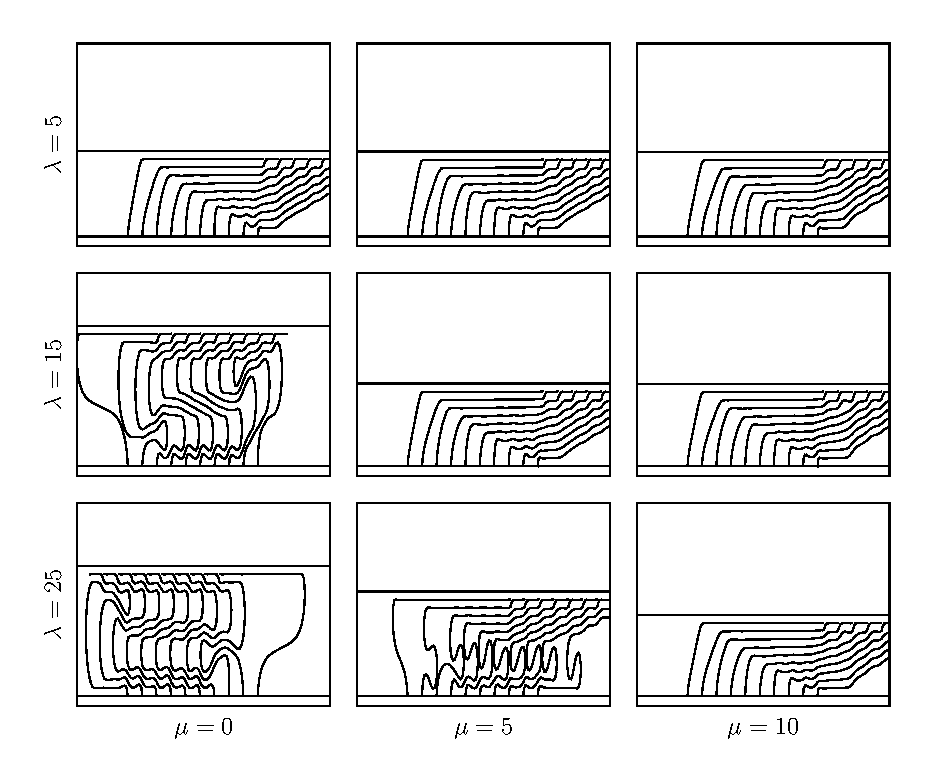
\includegraphics[scale=1]{./fig/ch4/grid.eps}
		\end{center}		
		\caption{Equilibrium configurations of ten fibers with 96 particles each for varying loads. The top left plot is a configuration with a load of $\lambda = 5$ and $\mu = 0$. The configurations immediately to the right are increasing $\mu$, and immediately below are increasing $\lambda$. All configurations use the reference parameters in Table~\ref{table:manyfiber_reference}.
		\label{fig:grid}}
	\end{figure}
	
	For computational reasons the granularity of our search space is signficantly smaller than with the single fiber case. We consider nine simulations with values of $\lambda = 5, 15, 25$ and $\mu = 0, 5, 10$. In Figure~\ref{fig:grid} we see a high level view of each simulation for the reference parameters. Keeping the horizontal component of the load zero, we see an increase in the aggregate curvature of all ten fibers as we increase $\lambda$. One explanation for this is that the torsional and extensible springs are not given enough leverage to slide along the top substrate and align to it. As the magnitude of the load is increased the fibers become more likely to buckle. If we increase $\mu$ the story changes. We are able to maintain the aligned compressed configuration for larger magnitudes of the load if the horizontal component is sufficiently large. It would seem the ratio between vertical and horizontal component for the reference parameters is the deciding factor for whether or not fibers will buckle.

	\begin{figure}
		\begin{center}
			\includegraphics[scale=1]{./fig/ch4/grid_b100.eps}
		\end{center}		
		\caption{Equilibrium configurations of varying loads. All configurations are directly comparable to Figure~\ref{fig:grid} with the exception that $\beta = 100$.
		\label{fig:grid_b100}}
	\end{figure}

	In Figure~\ref{fig:grid_b100} we increase $\beta$ to one hundred. This is an order of magnitude increase from the reference parameters and prevents any buckling at all for the loads we have selected. Qualitatively it is hard to see any difference in any of the nine simulations with the one exception that the fibers buckle to the left with no horizontal component. This bias with a load that has no horizontal component could be caused by a numerical artifact or an asymmetry in the number of atoms on the top substrate to the left of the leftmost fiber versus to the right of the rightmost fiber. Regardless of the reason the configuration itself is close enough to a reflection of the other configurations with a nonzero horizontal component that it would seem negligible.
	
	\begin{figure}
		\begin{center}
			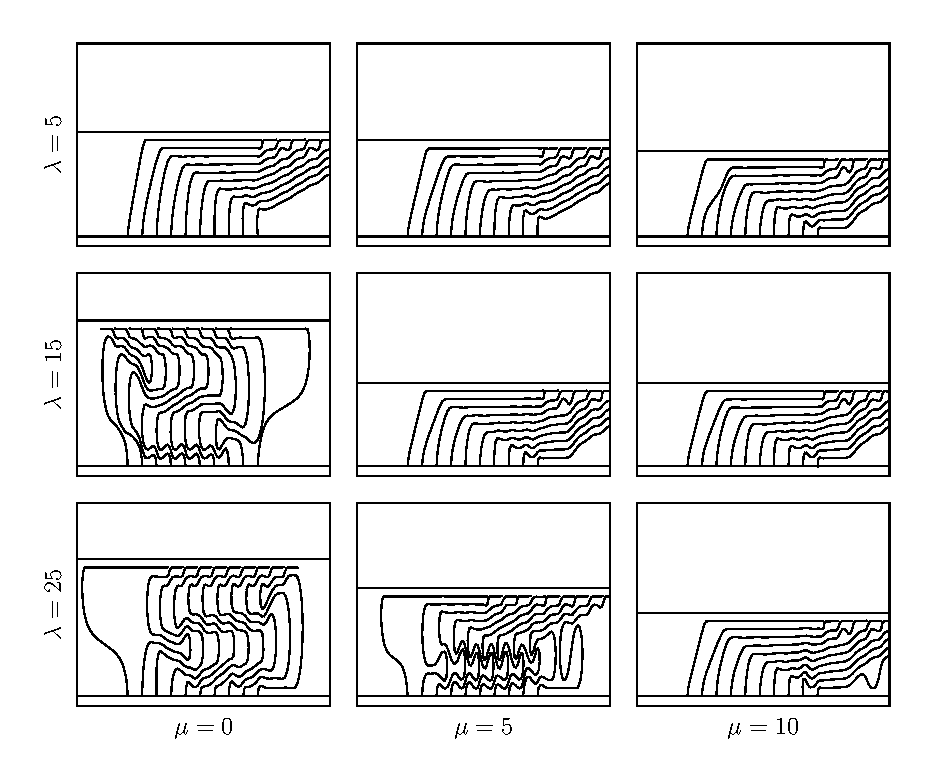
\includegraphics[scale=1]{./fig/ch4/grid_g1000.eps}
		\end{center}		
		\caption{Equilibrium configurations of varying loads. All configurations are directly comparable to Figure~\ref{fig:grid} with the exception that $\gamma = 1000$.
		\label{fig:grid_g1000}}
	\end{figure}
	
	Although the increase in the torsional spring strength was too much to allow for any interesting buckling to happen, an order of magnitude increase in the extensible spring constant does not seem qualitatively significant at all. Comparing Figure~\ref{fig:grid_g1000} to Figure~\ref{fig:grid} the same regime of configurations is present in both. With $\gamma$ sufficiently large and vdW sufficiently weak, all else held constant, further increasing $\gamma$ would play  a negligible effect because the distance between particles on a fiber is already close to $\ell$. It would seem, at least for our reference parameters, that this is the situation we are in when increasing $\gamma$ to 1000.
	
	\begin{figure}
		\begin{center}
			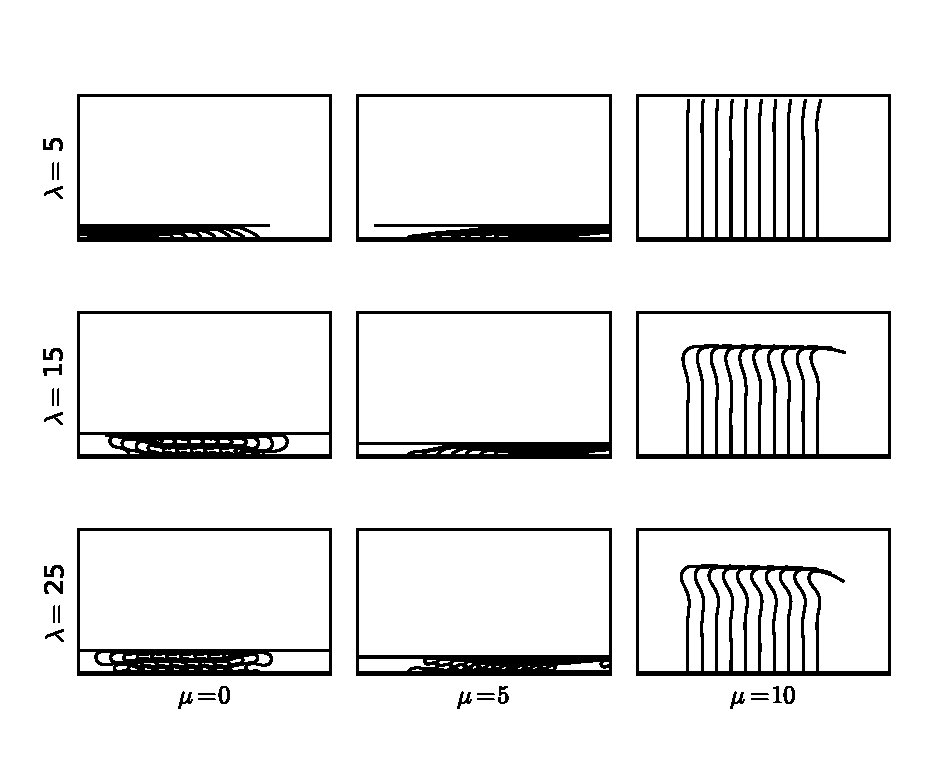
\includegraphics[scale=1]{./fig/ch4/grid_et0.1.eps}
		\end{center}		
		\caption{Equilibrium configurations of varying loads. All configurations are directly comparable to Figure~\ref{fig:grid} with the exception that $\eps_+ = 0.1$.
		\label{fig:grid_et0.1}}
	\end{figure}

	More interestingly we can consider the asymmetry present in the vdW strengths in our reference parameters. That is, $\eps = \eps_- = 0.1$, but $\eps_+ = 1$. In Figure~\ref{fig:grid_et0.1} we reduce $\eps_+$ to 0.1 and observe the results four our small case of simulations. For $\mu = 0$ or $5$ the situation is comparable to the reference parameters although the buckling for large magnitudes of the load with sufficiently weak horizontal component is different. What is more obvious though is that the horizontal component of the load can be too strong such that it simply slides off the fibers overpowering the vdW interaction. Moreover this happens for any value of the vertical component of the load. One would guess that if the vertical component is sufficiently strong you would find yourself in a situation similar to the propagating waves in the detachment experiment of Chapter~\ref{chap:three}.
	
	We perform the detachment experiment on a configuration of many fibers in large part as a proof of concept that the model scales up. However these play simulations do not fully demonstrate the benefit of scale you can obtain with the simplicity of the model we have presented. Ideally such a model is so simple \textit{because} you want to explore very large systems under the assumption the model will be approximately correct or insightful in some way.


	